\documentclass[../main.tex]{subfiles}
\usepackage{xifthen}
\newcommand{\etat}[1]{\left| #1 \right\rangle}
\newcommand{\etatF}[2]{\etat{ F=#1 \ifthenelse{\isempty{#2}}{}{,m_{\mathrm{F}}=#2} }}
\newcommand{\gftilde}[0]{\widetilde{g}_{\mathrm{F},m_{\mathrm{F}}}}
\newcommand{\mf}[0]{m_{\mathrm{F}}}
\newcommand{\mub}[0]{\mu_{\text{B}}}
\newcommand{\deltahf}[0]{\Delta_{\mathrm{hf}}}
\newcommand{\magicB}[0]{B_0^*}

\begin{document}

\chapter{Mises à jour de l'expérience}
\label{ch:new_exp}

Nous avons vu dans le chapitre précédent comment, expérimentalement, nous pouvons créer une onde de matière obtenue par la condensation de Bose-Einstein. Nous avons ainsi présenté les principaux outils dont nous disposons pour manipuler les atomes et la manière dont nous en tirons profit sur notre dispositif. Une telle plateforme recquiert une quantité importante de matériels variés qu'il est nécessaire d'entretenir, de réparer, voire de remplacer. 

Dans ce nouveau chapitre, nous nous pencherons sur les modifications apportées à l'expérience au cours de ma thèse. Dans la première partie, nous parlerons d'informatique et plus particulièrement du contrôle de l'expérience. Dans un second temps, nous caractériserons la lévitation magnétique suite à une avarie sur le circuit de refroidissement à eau. Ensuite, nous calibrerons le piège dipolaire dont le laser source a été changé. Pour terminer, nous discuterons de l'amélioration de l'évaporation optique permise par les changements précédents.

\section{Contributions au système informatique de l'expérience}
Souvent absente des présentations des expériences, l'informatique occupe pourtant une place primordiale dans les dispositifs d'atomes ultra-froids. Le contrôle simultané et de manière séquentielle des différents équipements de l'expérience, souvent précis à la micro-seconde, n'est possible qu'à l'aide d'un ordinateur disposant de sorties de tension controllables. Cet ordinateur, appelé \emph{séquenceur}, constitue le cerveau de l'ensemble du dispositif et contrôle tous les éléments nécessaires à la manipulation des atomes.

Le second aspect où l'informatique se rend indispensable réside dans l'acquisition et le traitement d'images. Le contrôle des caméras et l'extraction des quantités physiques à partir d'images expérimentales nécessite l'utilisation d'un ordinateur et d'au moins un logiciel adapté. 

De manière générale, les ordinateurs sont les éléments du dispositif avec lesquels l'expérimentateur intéragit le plus. Dans cette partie, on présentera donc les changements informatiques ayant eu lieu durant ma thèse.

\subsection{Contrôle de l'expérience: passage à la suite Cicero}
\label{sc:cicero}
Une modification majeure a été le changement du séquenceur de l'expérience. Le précédent système développé par André Villing, ingénieur électronicien du laboratoire maintenant retraité, était piloté de manière programmatique depuis le logiciel Matlab. À des fins de maintenance ansi que de meilleures performances, le nouveau séquenceur est d'origine commerciale et est basé sur du matériel \emph{National Instruments}:
\begin{itemize}
\item[\textendash] Un ordinateur \emph{PXIe-8840} dans un chassis \emph{PXIe-1078} qui alimente aussi les cartes de génération de signaux.
\item[\textendash] Deux cartes numériques \emph{PXIe-6535} de 32 voies chacune.
\item[\textendash] Deux cartes analogiques \emph{PXIE-6738} de 32 voies $\pm10$V chacune et codées sur 16 bits.
\end{itemize}
En addition, un circuit logique programmable (\emph{FPGA}) \emph{XEM3001} provenant de \emph{Opal-Kelly} permet de générer une horloge de fréquence variable pour le matériel \emph{National Instruments}. La justification de cette horloge de fréquence variable réside dans la grande variabilité de la durée des différentes étapes d'une expérience d'atomes ultra-froids: l'expérience peut rester dans le même état plusieurs secondes (pendant le chargement d'un MOT par exemple) tout comme elle doit pouvoir changer d'état pendant quelques microsecondes seulement (pendant l'imagerie par exemple). Une séquence durant typiquement 30s discrétisée toutes les microsecondes pour un minimum d'une cinquantaine de voies saturerait alors la mémoire de l'ordinateur. 

L'écriture de la séquence se fait à présent grâce à la suite \emph{Cicero Word Generator}, développée au \emph{MIT} dans le groupe de Wolfgang Ketterle \citep{keshet2013distributed}. Cette suite comporte deux logiciels qui fonctionnent selon une architecture client/serveur. Le client \emph{Cicero} est une interface graphique dans laquelle l'utilisateur écrit une séquence sous la forme d'une suite d'étapes comme illustré figure \ref{fig:cicero}. Au lancement d'un cycle expérimental, \emph{Cicero} envoie les données de séquence au serveur \emph{Atticus} qui calcule alors les consignes des cartes ainsi que l'horloge variable à appliquer \citep{keshet2008cicero}.

\begin{figure}
\centering
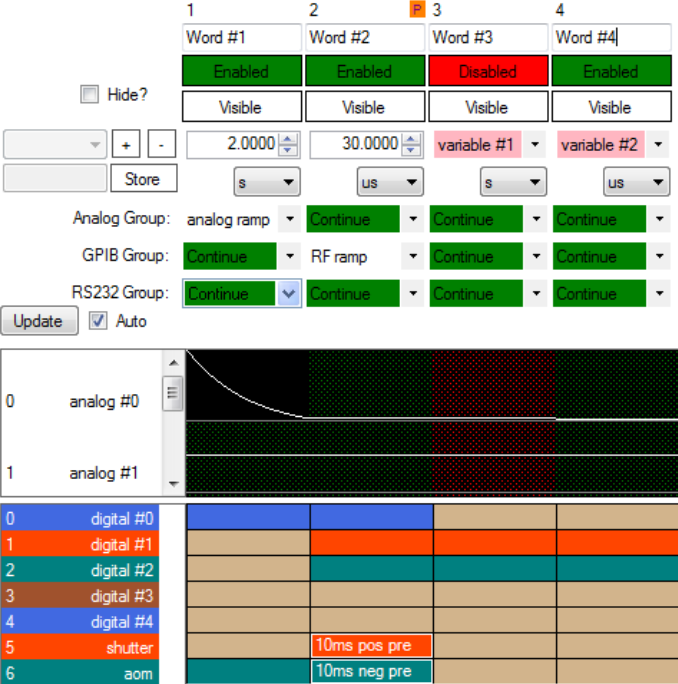
\includegraphics[width=0.7\textwidth]{../Fig/Modif_exp/cicero.png}
\caption{\textbf{Capture d'écran de \emph{Cicero}.} Une séquence est une suite d'étapes (des colonnes dans l'interface) pendant lesquelles on peut faire des motifs avec les voies analogiques. Les voies numériques changent d'état en général entre deux étapes. Il est possible de désactiver certaines étapes et d'utiliser des variables. Figure tirée de \citep{keshet2013distributed}.}
\label{fig:cicero}
\end{figure}

Grâce à cette architecture client/serveur, il est possible de connecter une interface \emph{Cicero} à plusieurs serveurs. Nous avons ainsi développé un serveur supplémentaire\footnote{Une attention particulière a été accordée à n'apporter aucune modification au code source de la suite \emph{Cicero} excepté dans l'environnement de ce serveur. Les environnements de \emph{Cicero}, \emph{Atticus} et les environnements communs n'ont subit aucun changement pour s'assurer de la compatibilité avec la version compilée 1.64rev7 de la suite.} afin de faciliter notre traitement de données. Celui-ci enregistre les principales données de séquence\footnote{Il s'agit du nom de séquence, de l'heure de lancement, de l'ensemble des variables, des étapes, des groupes d'étapes et de la dernière consigne du piège dipolaire avant le temps de vol.} à chaque cycle.

Ce changement de séquenceur ouvre de nouvelles perspectives en augmentant le nombre de voies utilisables (16 voies analogiques codées sur 12 bits et 48 voies numériques avec le précédent système) tout en permettant la génération de signaux arbitraires (auparavant limités à des morceaux de rampes).


\subsection{Développement d'une nouvelle interface d'acquisition et de traitement d'images}
Comme présenté dans la partie \ref{sc:imagerie}, les caméras que l'on utilise sur l'expérience sont configurées et contrôlées via le logiciel Matlab. En particulier, l'acquisition et le traitement des images se faisait à l'aide d'une interface commune avec l'ancien séquenceur. Son remplacement a donc eu un impact important sur le fonctionnement de la partie imagerie. 

En conséquence, nous avons réalisé une nouvelle interface graphique permettant de configurer les caméras, d'acquérir et de traiter les images, d'enregistrer les données et de contrôler tout les éléments non adressables depuis \emph{Cicero}. Le cahier des charges de cette nouvelle interface est donc le suivant:
\begin{itemize}
\item[\textendash] Gestion des trois caméras, avec possibilité de faire l'acquisition simultanée sur les deux caméras de la chambre de science\footnote{Un ordinateur supplémentaire était nécessaire pour le contrôle de la caméra \textit{bottom}, pilotée via une autre interface. Il fallait donc synchroniser ces deux ordinateurs qui enregistraient chacun leurs fichiers de données.}.
\item[\textendash] Imagerie par absorption et par fluorescence.
\item[\textendash] Calcul en direct des grandeurs physiques pour chaque image.
\item[\textendash] Lecture des données de Cicero récupérées grâce au serveur que nous avons développé.
\item[\textendash] Programmation en début de cycle des sources radio-fréquence utilisées pour l'évaporation radio-fréquence et la manipulation de l'état de spin dans la chambre de science\footnote{Cette programmation en début de cycle est rendue possible grâce à l'utilisation d'un \emph{FileSystemWatcher} provenant d'une bibliothèque .NET utilisable dans Matlab. Un fichier texte contenant les données du cycle en cours est généré en début de séquence par le serveur que nous avons développé, déclenchant alors automatiquement sa lecture par l'interface.}.
\item[\textendash] Enregistrement de l'ensemble des données et des paramètres du cycle pour un futur traitement.
\end{itemize}
L'utilisation de cette nouvelle interface a donc permit de centraliser les données générées par l'acquisition d'images en n'ayant plus besoin d'un ordinateur supplémentaire (et de la synchronisation associée). De plus, ce changement a permit de s'affranchir de plusieurs canaux de communication, les libérant ainsi pour le contrôle d'instruments. Enfin, l'utilisation et le fonctionnement de cette nouvelle interface Matlab sont simplifiés, permettant d'opérer avec une plus grande facilité les changements à venir sur l'expérience.











\section{Calibration de la lévitation magnétique}
\label{sc:levitation}
Comme présenté partie \ref{sc:chambre_science}, la lévitation magnétique est un élément essentiel de notre expérience. En plus d'être un pré-requis pour l'étude de la localisation d'Anderson à trois dimensions, celle-ci nous permet de manière générale d'obtenir des échantillons particulièrement froids. Son bon fonctionnement est donc une priorité pour notre expérience.

Malheureusement, une avarie dans le circuit de refroidissement de la lévitation a conduit à son démontage. Les modifications apportées avant remontage ayant pu conduire à une modification du comportement magnétique du système, une nouvelle calibration des champs générés a été menée.

Dans cette partie, nous présenterons dans un premier temps notre système de lévitation ainsi que les modifications qui y ont été apportées. Ensuite, nous nous pencherons sur les méthodes utilisées pour calibrer le système après sa réinstallation sur l'expérience, en commençant par des expériences d'oscillations puis à l'aide transitions radio-fréquences.




\subsection{Implémentation de la lévitation magnétique}

L'ensemble du système de la lévitation magnétique a été développé alors que l'équipe se dirigeait vers les expériences de localisation d'Anderson à trois dimensions. De nombreux détails de conception pourront être retrouvés dans le manuscrit de thèse d'Alain Bernard \citep{bernard2010transport}, mais rappelons les éléments nécessaires à la suite.

La lévitation magnétique est composée de plusieurs bobines collées dans un support en aluminium, qui sert aussi de réservoir thermique à l'aide d'un refroidissement à eau. Après de lourds travaux de débouchage et d'étanchéité, ce refroidissement est à présent effectué par le contact entre le support en aluminium et la circulation d'eau dans deux tubes en cuivre encastrés\footnote{Auparavant, l'eau circulait directement dans des trous percés dans le support en aluminium. Le débouchage de ces trous leur a fait perdre leur étanchéité, et après quelques essais infructueux, nous avons retenu la solution de deux tubes de cuivre encastrés et débouchants. De nombreux tests électriques ont été menés sur les bobines tout au long de leur maintenance pour s'assurer de l'absence de dégradation.}. L'efficacité de ce refroidissement est illustrée figure \ref{fig:refroidissement_levitation}.

\begin{figure}
\centering
\includegraphics[width=\textwidth]{../Fig/Modif_exp/levitation_refroidissement.pdf}
\caption{\textbf{a: Refroidissement de la lévitation magnétique.} L'un des supports des bobines de la lévitation est maintenant refroidi à l'aide de deux tubes en cuivre le traversant. Auparavant, l'eau circulait directement dans le support dans un circuit percé illustré par les traits rouges. Les tubes en cuivre ont pu être installés en rendant une partie de ce circuit débouchant. \textbf{b: Efficacité de refroidissement.} Ces mesures ont été réalisées dans des conditions proches de véritables cycles expérimentaux. Le même courant a été appliqué pendant 10s sur toutes les bobines à la fin de séquences habituelles. La température a été mesurée après la répétition d'au moins 30 cycles et en s'assurant de sa stabilisation.}
\label{fig:refroidissement_levitation}
\end{figure}


Ces supports, disposés de part et d'autre de la cellule, comportent chacun trois bobines. Les deux paires de bobines les plus proches de la cellule créent un champ de biais au niveau des atomes, dans des configurations légèrement plus rapprochée que celle de Helmholtz pour les bobines les plus proches de la cellule et légèrement plus éloignée pour les autres\footnote{L'intérêt de cette configuration est de contrôler la courbure du champ au niveau des atomes indépendamment de la valeur du champ. Il suffit de jouer sur l'équilibre des courants dans les différentes paires de bobines pour changer la courbure.}. Enfin, la paire de bobines la plus éloignée permet de créer un gradient magnétique qui permet de lutter contre la gravité.

Le champ magnétique au niveau des atomes peut alors être écrit:
\begin{equation}
\mathbf{B}=\left( \frac{b'}{2}x \right) \vec{x} + \left[ B_0 - b'y + b'' \left( y^2 - \frac{x^2+z^2}{2} \right) \right] \vec{y} + \left( \frac{b'}{2}z \right) \vec{z}
\end{equation}
où $b'$ correspond au gradient magnétique généré par les bobines de \emph{Gradient}, les plus éloignées de la cellule. Le  paramètre $b''$ est la courbure du champ généré par l'écart des bobines de \emph{Biais} à la configuration de Helmholtz. 
Le potentiel magnétique étant proportionnel à la norme du champ, celle-ci est donnée à l'ordre deux par
\begin{equation}
B=B_0 -b' y + b'' y^2 +\frac{1}{2} \left( \frac{b'^2}{4 B_0} - b'' \right) \left( x^2 + z^2 \right) 
\label{eq:norme_levitation}
\end{equation}
où le terme linéaire est celui qui permet de compenser la gravité.



Comme mentionné précédemment, il existe une limite pour les fréquences de piégeage (formule \ref{eq:theoreme_wing}) qui décroît avec la norme du champ magnétique. Une stratégie usuelle est donc de créer un champ aussi fort que possible, qui est d'environ 2000G avec notre système. Pour de tels champs, le potentiel magnétique n'est plus décrit par l'effet Zeeman linéaire, mais par la formule de Breit-Rabi \ref{eq:Breit-Rabi}. En revanche, pour une petite zone autour du centre de la lévitation, on peut simplifier l'étude en supposant que le champ change peu $B\simeq B_0$. On peut ainsi définir un facteur de Landé local
\begin{equation}
\gftilde(B_0)=\frac{1}{\mf \mub} \frac{\mathrm{d}E}{\mathrm{d}B}(B_0)
\end{equation}
obtenu à l'aide d'un développement limité de la formule de Breit-Rabi. La physique derrière cette approche est de considérer l'effet Zeeman linéaire sur un état dont la réponse dépend du champ de Biais $B_0$. La valeur du gradient nécessaire pour compenser la gravité peut alors être donnée par:
\begin{equation}
b'=\frac{mg}{\mf \gftilde(B_0) \mub}
\end{equation}
Cette dépendance est illustrée figure \ref{fig:levitation_etats} pour les différents états internes d'intérêt dans cette thèse: $\etatF{1}{-1}$, $\etatF{2}{+1}$ et $\etatF{2}{-2}$. Notons trois résultats remarquables: 
\begin{itemize}
\item[\textendash] L'état $\etatF{2}{-2}$ nécessite un gradient indépendant du biais magnétique pour être lévité.
\item[\textendash] Les états $\etatF{1}{-1}$ et $\etatF{2}{+1}$ sont lévités pour le même gradient à bas champ.
\item[\textendash] L'état $\etatF{1}{-1}$ ne peut être lévité qu'à bas champ, le gradient nécessaire pour contrer la gravité augmentant avec le champ magnétique.
\end{itemize}
Plusieurs stratégies expérimentales de lévitation s'offrent alors. La première provient de l'état $\etatF{2}{-2}$ qui peut être lévité tout en gardant la valeur du champ de biais comme un dégré de liberté, on peut alors réaliser des lévitations très décomprimées. Il s'agit de l'approche utilisée pour la mesure du temps de diffusion élastique, présentée chapitre \ref{ch:TauS_PRL}. Une autre possibilité est que les états $\etatF{1}{-1}$ et $\etatF{2}{+1}$ peuvent coexister dans le champ de lévitation, on peut ainsi utiliser l'état interne de l'atome comme degré de liberté tout en étant lévité. Cette stratégie a par exemple été utilisée pour la mesure des fonctions spectrales \citep{volchkov2018measurement}.

\begin{figure}
\centering
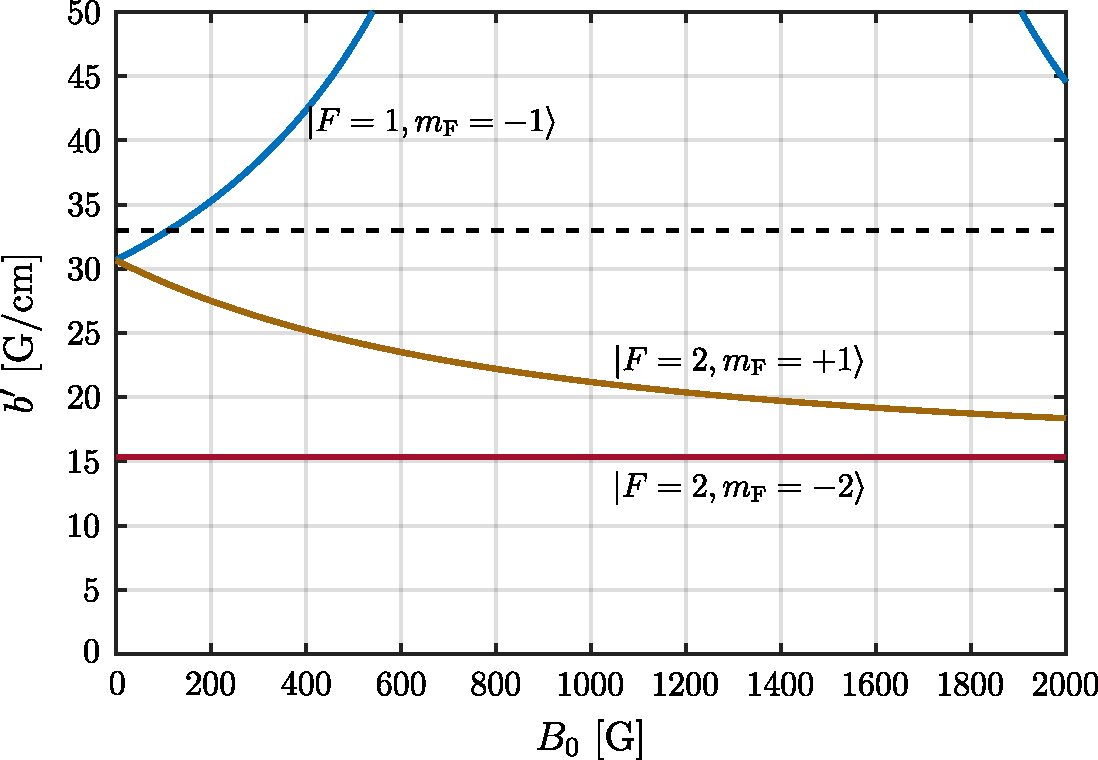
\includegraphics[width=0.8\textwidth]{../Fig/Modif_exp/levitation_etats.pdf}
\caption{\textbf{Gradient nécessaire pour compenser la gravité.} La valeur du gradient magnétique à appliquer pour léviter dépend de l'état électronique, mais aussi du biais magnétique $B_0$ par la formule de Breit-Rabi. L'état $\protect\etatF{1}{-1}$ ne peut être lévité qu'à bas champ, l'alimentation des bobines de gradient ne pouvant délivrer plus de 50A (limite tracée en pointillés).}
\label{fig:levitation_etats}
\end{figure}









\subsection{Calibration par radio-fréquences}
Cette dernière stratégie rend possible l'approche novatrice de désordre dépendant de l'état interne, qui impose de travailler à un \emph{biais magique} $\magicB=3.229G$ pour lequel les susceptibilités magnétiques des états $\etatF{1}{-1}$ et $\etatF{2}{+1}$ sont identiques \citep{denechaud2018vers}. La valeur précise de ce champ magique demande une connaissance fine des caractéristiques du dispositif de génération des champs magnétiques de l'expérience.

À ces fins, la mesure précise de ces champs magnétiques a été effectuée par spectroscopie radio-fréquence. Son principe repose sur le transfert de population entre l'état d'origine $\etatF{1}{-1}$ et les états $\lbrace \etatF{2}{-2},\etatF{2}{-1},\etatF{2}{0} \rbrace$ accessibles, dont la séparation en énergie dépend du champ magnétique. Ainsi, lorsque la radio-fréquence satisfait la condition de résonance $\nu_{\mathrm{RF}}=\deltahf + \delta \nu (B)$ avec $\delta \nu (B)$ le décalage par effet Zeeman, une partie des atomes sera transférée dans l'un des sous-états de $\etatF{2}{}$. Le principe de cette spectroscopie est illustré figure \ref{fig:calibration_RF}.

\begin{figure}
\centering

\caption{\textbf{Calibration par radio-fréquences}. Principe de la calibration des champs de biais à l'aide de radio-fréquences.}
\label{fig:calibration_RF}
\end{figure}








imager uniquement les atomes dans $\etatF{2}{}$, ils se trouvent à l'origine dans $\etatF{1}{}$.
Possible car les déplacements lumineux dans l'ODT sont identiques pour les états $\etatF{1}{}$ et $\etatF{2}{}$ étant donné le désaccord du faisceau de pigégage.


caractérisation complète du champ rayonné par les 2 biais et les deux compensations horizontales. possibilité d'extraire le champ naturellement présent. Utilisation des 7 sept transitions. 












\subsection{Etude du piégeage}
\label{sc:oscillations_levitation}
Il est primordial que les atomes se trouvent au centre de la lévitation car il s'agit de l'endroit où le champ magnétique est le plus homogène, et cette condition est d'autant plus importante alors nous nous orientons vers des lévitations à bas champ. En effet, c'est à bas champ que le piégeage de la lévitation est le plus important, c'est à dire que le champ est le plus inhomogène. 

\paragraph*{Fréquences de la lévitation}
D'autre part, si les atomes ne sont pas au centre du piège, la réalisation de temps de vol en présence de la lévitation conduira à un mouvement du nuage. Pour l'état $\left| F=1, m_{\mathrm{F}}=-1 \right\rangle$ en particulier, le centre de masse du nuage décrit des oscillations autour du centre de la lévitation dont les fréquences peuvent être trouvées à l'aide de la norme du champ magnétique \ref{eq:norme_levitation}:
\begin{equation}
\omega_x^2=\omega_z^2=\left| \frac{\mf \gftilde \mub}{m} \left( \frac{b'^2}{4 B_0} - b'' \right) \right|
\quad \text{et} \quad
\omega_y^2= \left| \frac{2 \mf \gftilde \mub }{m} b'' \right|
\end{equation}
L'exploitation de ces oscillations fournit donc de précieux renseignements quant à la position du centre de la lévitation, mais aussi quant à la forme du potentiel magnétique dans lequel les atomes évoluent. 

Il est possible d'obtenir une calibration du gradient à l'aide de la figure \ref{fig:levitation_etats}.  estimation correcte de la calibration des bobines de gradient à l'aide de paires gradient/biais qui permettent de compenser correctement la gravité.

Pour les études à bas-champ menées, on peut estimer la calibration des bobines de biais à l'aide des fréquences d'oscillations. L'étude des oscillations en fonction du biais permet d'extraire aussi la courbure.





\paragraph*{Centre de la lévitation}
Déplacement du centre de la lévitation à l'aide de champs de compensation.
\begin{equation}
\mathbf{B}=\left( \frac{b'}{2}x \right) \vec{x} + \left[ B_0 - b'y + b'' \left( y^2 - \frac{x^2+z^2}{2} \right) \right] \vec{y} + \left( \frac{b'}{2}z +B_z \right) \vec{z}
\end{equation}
\begin{equation}
z_c =-\frac{2B_z}{b'}\left( \frac{1}{1-4B_0 b'' /b'^2} \right)
\end{equation}
À bas champ, le déplacement n'est dû qu'au gradient et au champ de compensation. Avec un gros biais par contre, on doit prendre en compte les effets de la courbure. en particulier, il est possible d'expulser le centre de la lévitation à l'infini, ça arrive quand la fréquence $\omega_z$ s'annule.
effets de champs de biais de compensation.

Augmentation du biais induit un déplacement horizontal si on n'est pas au centre de la lévitation et si on change le gradient de sorte à compenser le changement de biais. Pour une étude résolue en énergie, sans force toussa toussa, il faut aussi changer le champ de biais de compensation. 





Cette étude a permis non seulement de calibrer nos bobines dont la position, l'orientation et le comportement magnétique ont été légèrement modifiés. Mais en plus, ça nous a permit de découvrir de nouvelles limitations. 
Future nécessité de pouvoir changer les courants de compensation de manière totalement arbitraire et contrôlée en cours de séquence non réalisable avec nos alimentations actuelles: étude en cours. 












\section{Changement du laser telecom et calibration du piège optique}
Listés dans la partie \ref{sc:chambre_science}, uniquement deux éléments participent à la manipulation d'atomes dans la chambre de science avant condensation. Le premier élément, la lévitation magnétique, a fait l'objet d'un entretien essentiel présenté dans la partie précédente. 

Cette partie se concentrera sur le second élément, le piège optique. Nous commencerons par présenter le système optique et décrire les changements opérés, puis nous décrirons la calibration de ce piège sur les atomes.

\subsection{Changement du laser telecom}
Dans le chapitre précédent, nous avons vu que le piège dipolaire était composé de deux faisceaux se croisant dans la chambre de science. Ces deux faisceaux, la pince et le dimple, sont orientés suivant les directions $\vec{z}$ et $\vec{y}$ respectivement et permettent de franchir le seuil de condensation. Il s'agit donc du piège donnant au condensat ses propriétés. De plus, c'est avec ce même piège que l'on met en oeuvre les techniques de refroidissement extrême que sont l'ouverture adiabatique du piège ou encore le refroidissement par delta-kick. Il est donc primordial d'avoir une connaissance complète des caractéristiques de ce piège.

Les deux faisceaux du piège dipolaire croisé proviennent d'une source laser commune avant d'être mis en forme séparément. Cette source, un laser fibré Ytterbium de \emph{Keopsys} émettant une puissance 20W en continu à une longueur d'onde $\lambda=1070$nm, a été changée au cours de ma thèse. Ce laser a été sujet à un grand nombre d'opérations de maintenance, et, dans les mois précédant son remplacement, il ne pouvait plus émettre que 14W lors de son allumage et seulement 12.5W en fin de journée.
 
Cette source a été remplacée par un laser fibré Ytterbium \emph{YLR-50-LP-A-Y12} de \emph{IPG}, opérant à la même longueur d'onde $\lambda=1070$nm, et avec une puissance maximale mesurée à 55W. La taille du faisceau en sortie de fibre est de 0.8mm (contre 1.4mm pour le laser Keopsys), il a donc fallu adapter un télescope afin de conserver les mêmes tailles de faisceaux au niveau des atomes. Le montage de mise en forme des faisceaux est présenté figure \ref{fig:optique_1070}. Celui-ci est majoritairement mis dans des tubes (représentés figure \ref{fig:optique_1070}) contenant un grand nombre de diaphragmes, facilitant ainsi la procédure d'alignement.

\begin{figure}
\centering
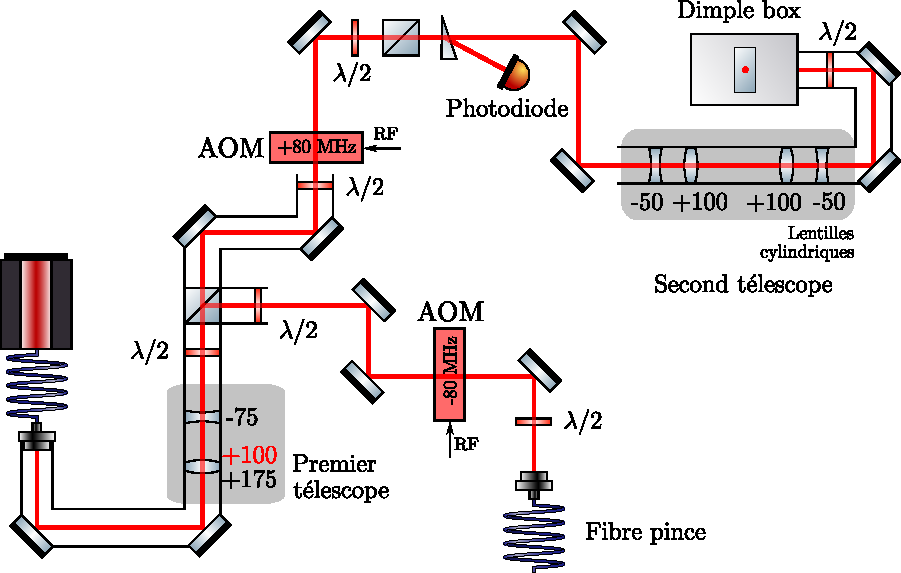
\includegraphics[width=0.9\textwidth]{../Fig/Modif_exp/optique_1070.pdf}
\caption{\textbf{Schéma du montage optique pour le piège dipolaire.} Le faisceau issu du laser source passe dans un premier télescope avant d'étre séparé en deux parties. La partie déviée passe dans une fibre optique pour devenir le faisceau de la pince. La partie transmise passe ensuite dans un second téléscope pour devenir elliptique et arrive dans la \emph{Dimple box}, qui envoie le faisceau sur les atomes et contient les optiques d'imagerie \citep{muller2015coherent}. Afin de garder les mêmes tailles de faisceaux, la première lentille du premier télescope a été remplacée par une lentille de focale +100mm.}
\label{fig:optique_1070}
\end{figure}


\subsection{Calibration du piège optique}
La présence d'une fibre optique pour la mise en forme du faisceau de la pince permet de s'assurer que le mode envoyé sur les atomes n'a pas changé. Pour le faisceau dimple en revanche, le trajet jusqu'à la cellule se fait sans filtrage. La présence de deux périscopes, d'un nombre d'éléments optiques important et l'utilisation d'un profil elliptique imposent une étude attentive des caractéristiques de ce faisceau au niveau des atomes.



\paragraph*{Estimation de la taille du faisceau au niveau des atomes}
Le faisceau dimple est rendu elliptique à l'aide du second télescope qui comporte quatre lentilles dont deux cylindriques, comme illustré figure \ref{fig:optique_1070}. Le rapport de forme du faisceau est alors de 2. Cependant, l'utilisation de plusieurs périscopes risque de faire tourner cette ellipse, il est donc primordial de connaître les tailles du faisceau au niveau des atomes.

L'approche suivie pour estimer le profil du faisceau au niveau des atomes consiste à en étudier la divergence après la cellule à l'aide d'une caméra, la zone d'intérêt se trouvant sous vide. Un avantage de cette méthode est de s'affranchir d'un système optique qui compliquerait le traitement, sous réserve que la caméra soit suffisamment large pour imager l'entièreté du faisceau. Le principal inconvénient est qu'il est nécessaire d'extrapoler la forme du faisceau pour en estimer le profil au niveau des atomes.

Cette extrapolation est en réalité aisée: la taille du faisceau $\mathrm{w}_{\mathrm{i}}(y)$ dans la direction $\vec{i}$ ($\vec{i}= \lbrace \vec{x},\vec{z} \rbrace$) est donnée par l'optique gaussienne:
\begin{equation}
\mathrm{w}_{\mathrm{i}}(y)=\mathrm{w}_{\mathrm{i}} \sqrt{1+\left( \frac{y}{y_{\mathrm{Ri}}} \right)^2}
\label{eq:taille_faisceau}
\end{equation}
où $\mathrm{w}_{\mathrm{i}}$ est le waist du faisceau dans la direction $\vec{i}$. La distance de Rayleigh associée s'exprime $y_{\mathrm{Ri}}=\pi \mathrm{w}_{\mathrm{i}}^2 / \lambda$ et correspond à la distance sur laquelle la taille du faisceau suivant la direction $\vec{i}$ change peu. Dans le régime de champ lointain $y \gg y_{\mathrm{Ri}}$, le faisceau diverge selon un angle $\tan \theta_{\mathrm{i}} \simeq \lambda / \pi \mathrm{w}_{\mathrm{i}}$.

La mesure des tailles du faisceau a été réalisée à l'aide d'une caméra \emph{IDS Ueye} disposant d'une matrice de $1024 \times 1280$ pixels de 5.2µm de côté. Les tailles ont été extraites par ajustement gaussien après integration suivant une direction. Enfin, l'évolution de la taille en fonction de la position a été ajustée par la formule \ref{eq:taille_faisceau}, illustrée figure \ref{fig:taille_dimple}.

\begin{figure}
\centering
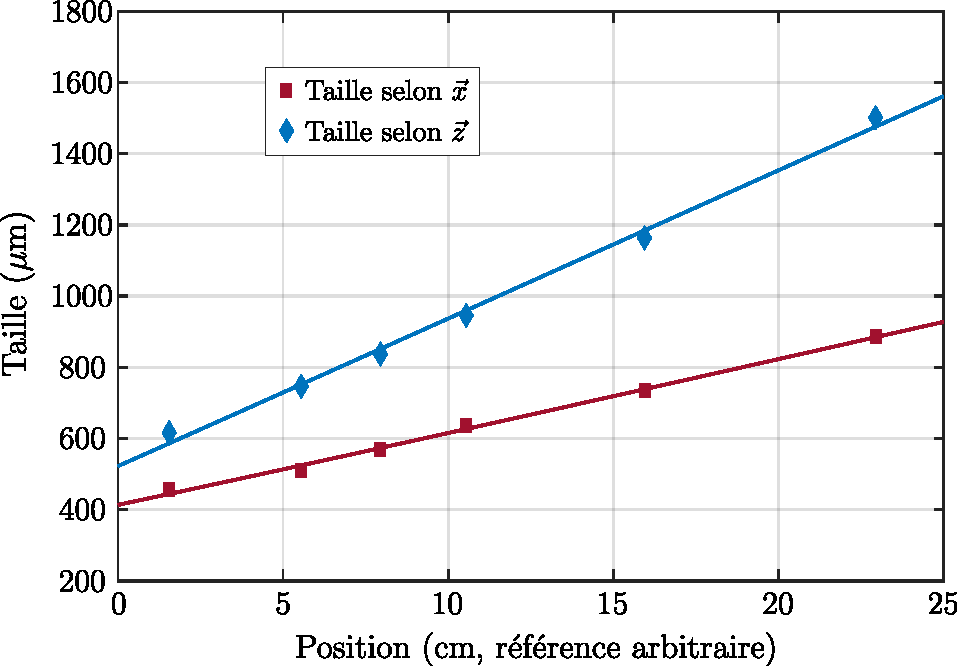
\includegraphics[width=0.8\textwidth]{../Fig/Modif_exp/expansion_dimple.pdf}
\caption{\textbf{Divergence du faisceau dimple après la cellule.} Les tailles du faisceau dimple sont représentées en fonction de la position de la caméra. La divergence du faisceau permet de remonter aux waists du faisceau et d'en estimer la position. Les waists extraits sont de $\mathrm{w_z}\simeq82$µm et de $\mathrm{w_x}\simeq160$µm et leur position est compatible avec celle des atomes.}
\label{fig:taille_dimple}
\end{figure}

On estime alors les waists du faisceau à $\mathrm{w_z}=81.6 \pm 7.8$µm et $\mathrm{w_x}=160\pm 13$µm, assez proche des valeurs précédentes. La position de ces waists est compatible avec la position des atomes, et la longueur de Rayleigh du faisceau est de l'ordre de $y_{\mathrm{Rz}}\simeq$2cm.








\paragraph*{Calibration des fréquences de piégeage}
Le fonctionnement du piège optique repose sur le potentiel dipolaire. Celui-ci s'écrit:
\begin{equation}
U(\mathbf{r})=\frac{3 \pi c^2 \Gamma}{2 \omega_0^3 \overline{\Delta}} I(\mathbf{r}) \quad \text{avec} \quad \frac{1}{\overline{\Delta}}=\frac{1}{\omega-\omega_0}-\frac{1}{\omega+\omega_0}
\end{equation}
En supposant que les atomes restent proches du centre du piège, on peut faire l'approximation que le profil d'intensité des faisceaux est de forme harmonique. On peut ainsi définir la profondeur de piégeage pour chaque faisceau:
\begin{equation}
U_{\mathrm{pince}}= \frac{3c^2 \Gamma }{\omega_0^3 \overline{\Delta}} \frac{P_{\mathrm{pince}}}{\mathrm{w}_0^2} \quad \text{et} \quad U_{\mathrm{dimple}}=\frac{3c^2 \Gamma }{\omega_0^3 \overline{\Delta}}\frac{P_{\mathrm{dimple}}}{\mathrm{w}_{\mathrm{x}} \mathrm{w}_{\mathrm{z}}}
\label{eq:profondeur_piege_optique}
\end{equation}
ainsi que les fréquences de piégeage $\omega_{x,y,z}$. Rappelons que le confinement dans les directions $\vec{x}$ et $\vec{y}$ est fait par la pince, et que celui dans la direction $\vec{z}$ est fait par le dimple, les fréquences de piégeage du piège dipolaire croisé s'expriment alors:
\begin{equation}
\omega_x=\omega_y=\sqrt{-\frac{4 U_{\mathrm{pince}}}{m \mathrm{w}_0^2}} \quad \text{et} \quad \omega_z=\sqrt{-\frac{4U_{\mathrm{dimple}}}{m \mathrm{w}_{\mathrm{z}}^2}}
\label{eq:frequences_piege_optique}
\end{equation}
La caractérisation finale du piège dipolaire croisé se fait à l'aide des fréquences de piégeage, qui fixent les propriétés physiques du nuage. Afin de mesurer ces fréquences, nous avons fait le choix d'induire de petites oscillations du nuage à l'intérieur du piège à l'aide d'une force extérieure, et de suivre ces oscillations en fonction du temps d'évolution dans le piège de manière équivalente à celle présentée pour la lévitation magnétique section \ref{sc:oscillations_levitation}. 

La fréquence de piégeage de la pince a été mesurée suivant la direction verticale à l'aide de la lévitation magnétique. En commutant rapidement le courant des bobines de gradient, on dispose d'un bouton pour allumer et éteindre la gravité, et donc générer une force pendant un bref instant pour donner un mouvement aux atomes dans le piège. En relevant la position des atomes en fonction de la durée d'évolution dans le piège après excitation, on extrait alors la fréquence associée.

La mesure de la fréquence de piégeage dans la direction $\vec{z}$, provenant du dimple, a été effectuée selon deux méthodes suivant la puissance du faisceau:
\begin{itemize}
\item[\textendash] À haute puissance, on pousse les atomes à l'aide d'un gradient magnétique provenant de bobines de compensation. Celles-ci peuvent pousser les atomes pendant de courts instants à l'aide d'un commutateur rapide.
\item[\textendash] À plus basse puissance, le piège optique est décomprimé et peu profond grâce à la lévitation. Cependant, le piégeage de la lévitation peut arracher les atomes du piège optique, il est donc nécessaire de déplacer le centre de la lévitation magnétique à l'aide de champs de compensation. Pour pousser les atomes, on utilise alors les bobines de compensation dans leur configuration normale, et leur brève extinction conduit à accélérer les atomes en déplaçant le centre de la lévitation magnétique.
\end{itemize}

L'ensemble de ces mesures est représenté figure \ref{fig:frequences_piege_optique}. La variation des fréquences s'est fait en abaissant la puissance du laser au cours de l'évaporation optique, celle-ci conduisant à une décompression du piège de comportement $\omega /2\pi =A \sqrt{P}$ comme illustré formules \ref{eq:profondeur_piege_optique} et \ref{eq:frequences_piege_optique}. Les fréquences mesurées expérimentalement (carrés pour la pince, losanges pour le dimple) sont comparées à celles estimées à l'aide de mesures de la puissance des faisceaux et de leurs tailles (lignes continues). Si la comparaison est tout à fait correcte pour la pince, ce n'est pas le cas pour le dimple qui présente une surestimation de la fréquence de piégeage. La calibration de la pince est alors $A_{\mathrm{pince}}=912\pm 30 \: \mathrm{Hz.W^{-1/2}}$, et celle du dimple est de $A_{\mathrm{dimple}}=62.5\pm 1.2 \: \mathrm{Hz.W^{-1/2}}$ . La prédiction pour cette dernière est de $103 \: \mathrm{Hz.W^{-1/2}}$ en utilisant les tailles mesurées $\mathrm{w}_{\mathrm{x}} \simeq 160 \mathrm{\mu m}$ et $\mathrm{w}_{\mathrm{z}} \simeq 82 \mathrm{\mu m}$, en accord qualitatif avec la valeur mesurée\footnote{La dernière calibration date de la mise en place de la \emph{dimple box} lors de la thèse de Kilian Muller \citep{muller2015coherent}. Celle du dimple était alors de $A_{\mathrm{dimple}}=64.5\pm 1.2 \mathrm{Hz.W^{-1/2}}$, très proche de la valeur actuelle.}. 

\begin{figure}
\centering
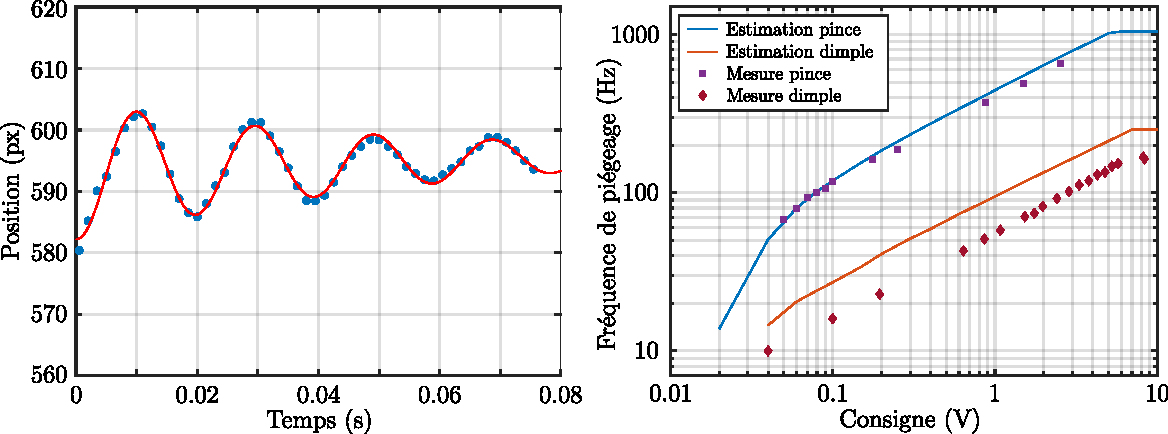
\includegraphics[width=\textwidth]{../Fig/Modif_exp/frequences_piege_optique.pdf}
\caption{\textbf{a: Exemple d'oscillation dans le piège optique.} Le nuage oscille dans la direction $\vec{z}$ pour une puissance du dimple de 0.70W après avoir été poussé par un gradient magnétique. La fréquence d'oscillation est alors de $\omega_z /2\pi \simeq 51 \: \mathrm{Hz}$. \textbf{b: Fréquences d'oscillations du piège optique.} Les fréquences mesurées par oscillations du nuage (points) sont comparées à des estimations issues de mesures de la taille des faisceaux et de mesures de puissance de ces faisceaux (lignes continues).}
\label{fig:frequences_piege_optique}
\end{figure}



Une seconde conséquence de la figure \ref{fig:frequences_piege_optique} est que les deux faisceaux présentent une saturation à haute puissance, c'est à dire qu'ils restent à leur puissance maximale au dela d'une certaine consigne seuil. Pour le dimple, cette saturation provient d'une limitation de la puissance de la source de la radio-fréquence servant à la diffraction du faisceau dans le modulateur acousto-optique. Pour la pince, cette limitation provient du maximum de l'efficacité de diffraction du modulateur acousto-optique. Ces deux saturations peuvent être repoussées en augmentant la puissance émise par le laser source\footnote{Le réglage actuellement utilisé sur l'expérience est une émission à 50\% de la puissance maximale du laser \emph{IPG}, c'est à dire environ 23W. Il a été observé que le mode émis est suffisamment stable à ce point de fonctionnement.}, cependant elles ne sont pas problématiques pour notre configuration. De plus, cette augmentation de puissance se traduirait par un chauffage local des bloqueurs de faisceau plus important, entraînant des effets thermiques néfastes.





\section{Optimisation de l'évaporation tout-optique}
\label{sc:evap_optique}


\end{document}